\documentclass[11pt, letterpaper]{article}
\usepackage{graphicx}
\title{Project 3: A Network Scheduler}
\begin{document}
\maketitle
\section{Administrative}

Team names: Rishi Dewan Lindsey O'Niell\\
Team uteids: rrd328 ldo252\\
Slip days previously used: 0\\
Slip days used this project: 0\\
Slip days remaining: 4\\

\section{Part 1: Basic synchronization}

{\em 
In order to implement Stats, we organized our data in two arrays. Both are of size $MAX\_FLOW\_ID + 1$ and the 
index corresponds to a flowID. 
One is called seenFlowID, which keeps track of whether or not the specified flowId has sent any data across 
the network. This way, in toString(...), we know at what point we need to 
stop adding to the buffer the values in our totalFlowID array, which keeps track of the total number 
of bytes each flowID has sent. 

update() continues to update the total number of bytes each flowID sends within
totalFlowID[] by adding the byteCount to the running total.  
It indicates if a flow has been seen before by setting seenFlowID[flowId]
to true. It also keeps track of the maxFlowID we have seen. 

In toString(), we decided to use sprintf(...) to handle our output. We simply iterate through our array of 
totalFlowIDs, adding the total number of bytes sent per flowId to our buffer. We keep a running total of the total from 
each flowID, which we concatenate to the end of the buffer after all of the individual flowID's byte values. 
}

\subsection{Evaluation}

\centerline{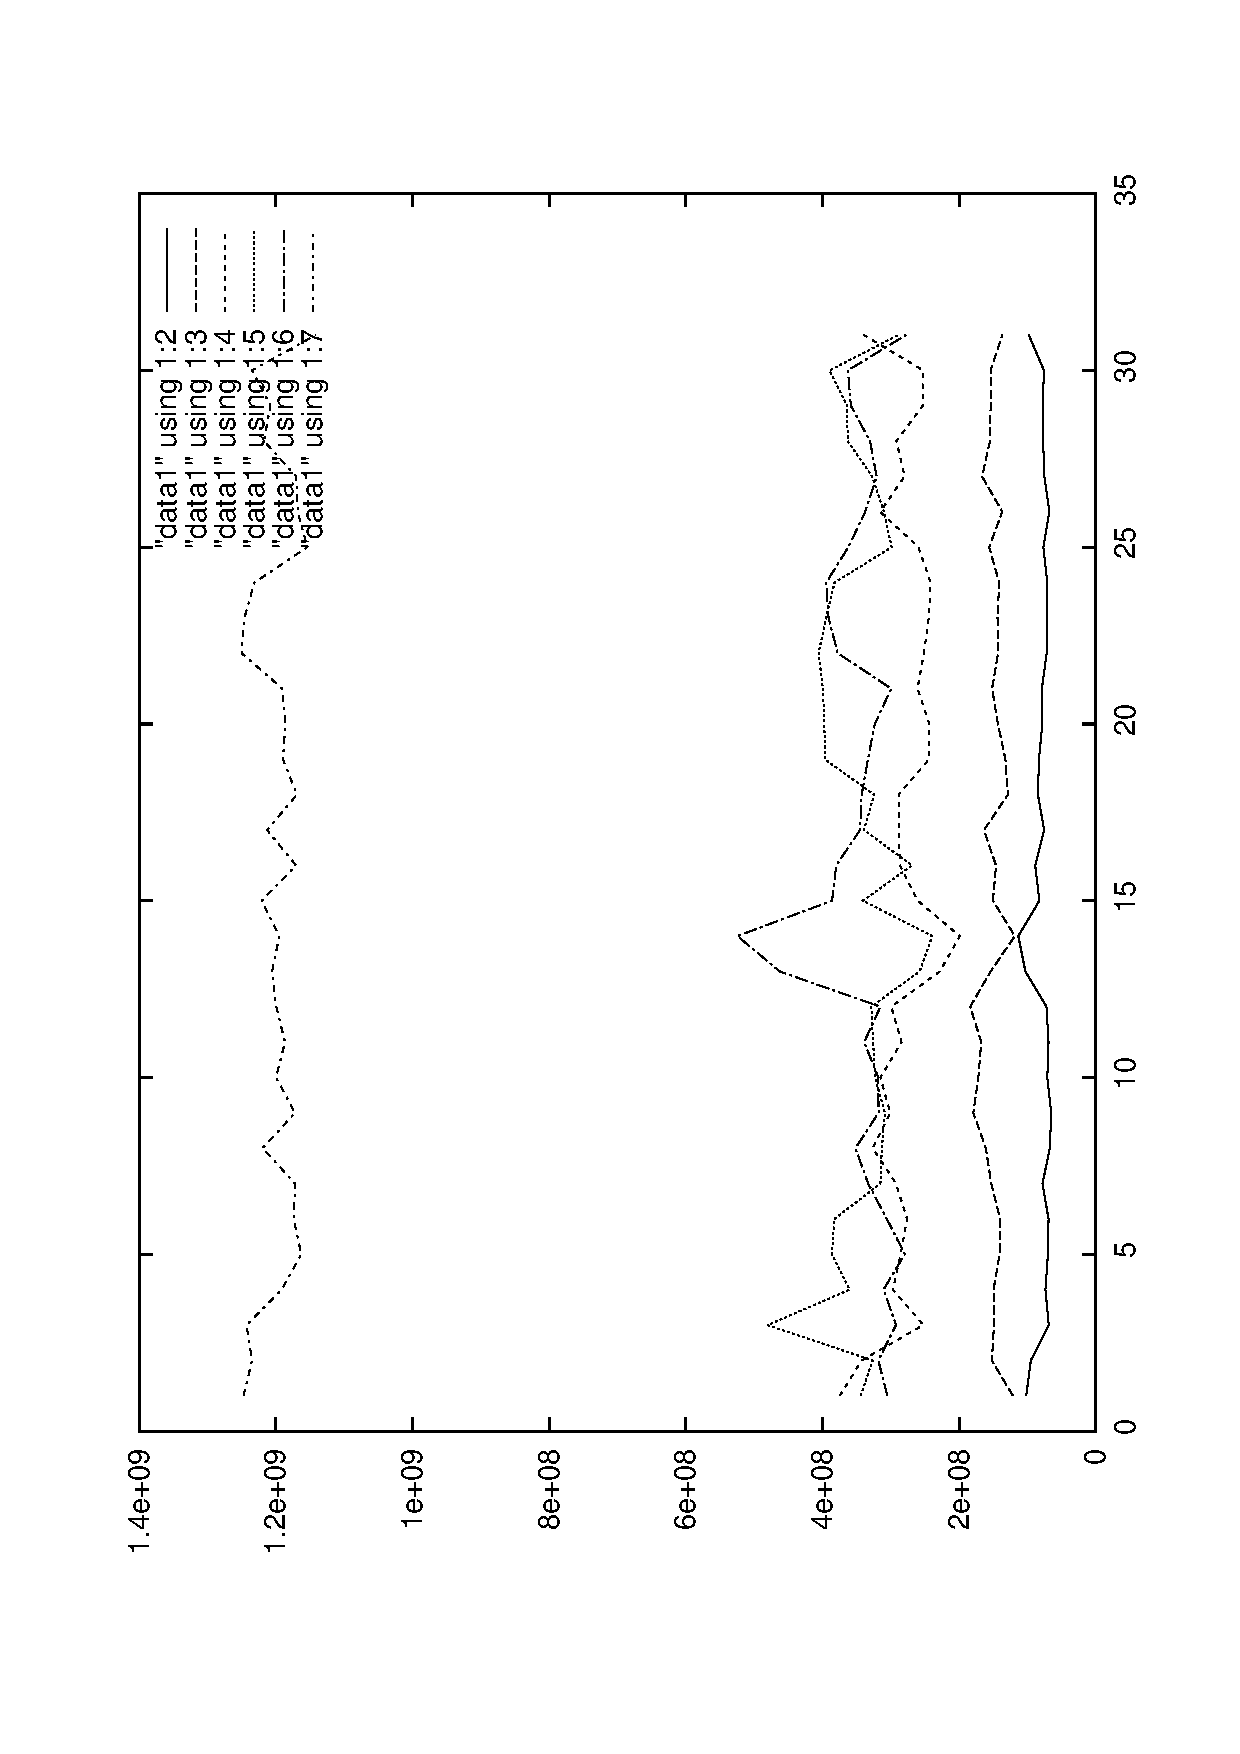
\includegraphics[width=3in]{plot1}}

{\em This graph indicates that given a pre-designated amount of threads (flows) to run, the
flows will attempt to send as many bytes through the socket as possible within the 1-second granularity.
Since the threads are sending an unlimited amount of bytes, the graph indicates each thread will send
a large number of bytes infinitely or until the network reaches a designated dieTime (in util.cc).}


\centerline{\includegraphics[width=3in]{plot1b}}

{\em The graph is basically similar to that of plot1, with the exception that now we have a
limited number of bytes to send over the socket. As before, the threads are sending as many bytes
as possible. However, with this new limit, the threads will eventually run out of bytes to send,
indicated by the large drop of the y-axis coordinates. It is not difficult to predict the time
interval in which the threads complete their tasks. Consider this instance, 2,000,000,000 bytes/thread are
being sent over the socket. 5 threads will result in 10,000,000,000 bytes to be sent. Based on the data from
data1b, the average amount of bytes sent in a second is 737,000,000. So, the predicted time it will take
to send all 10,000,000,000 bytes would be between 13-14 seconds.}

{\em Our tests are included in Stats.cc->unitTests().}



\section{Part 2: MaxNWScheduler}

{\em In MaxNWScheduler, we use one lock and two condition variables. The 
condition variable okToSend relates to when a flow is allowed to send 
its data. The condition variable alarmSignal makes the alarmThread wait 
until the next deadline is calculated before it continues running. 
We keep track of the maxRate, which is the limit on the number of bytes
that can be sent per second. We also have variables for the nextDeadline, 
current bytes being sent: currentBytes, and deadlineReached and deadlineCalculated,
which indicate if the current deadline has been reached and the next deadline
has been calculated, respectively. 

waitMyTurn(int ignoredFlowID, float ignoredWeight, int lenToSend): 
In this function, the current flow is made to wait to send its bytes until the 
network is free (the previously sending flow has reached its deadline). Once it 
is allowed to send, it calculates its deadline (nextDeadline), with the formula 
specified in the project page: 
$nextDeadline = currentTime + 1000*lenToSend/maxRate$. 
We then indicate that the current deadline has been calculated and has not yet 
been reached. We also signal the alarmThread, which has been waiting for the deadline
to be calculated in signalNextDeadline(...). 

signalNextDeadline(long long prevDeadlineMS): 
Upon entering the function, we indicate that the current flow has reached its deadline. 
We also indicate that the next deadline has not yet been calculated. We then signal 
that the network is free, so a flow waiting in waitMyTurn(...) is ok to send. Next, 
we make the alarmThread wait so that the current flow can calculate its next deadline. 
Once this is done, that deadline has not been reached (it was just set), and we return 
the nextDeadline.}

{\em For our testing strategy, we did some extra sendAndRecv's
(using our unit test file). The primary difference is we changed
the number of threads to run, as well as the dieTime in util.cc. We also calculated predicted amount
of seconds that each of the STFQ tests would last in terms of sending
all of its bytes.

Important: See the comments in the Makefile in the testPlot commands
(the comments show how many nflows will run as well at the maximum dieTime)}

{\em IMPORTANT: Our testing graphs included in this report were "made" with the specified 
nflows and dieTimes in the Makefile. If you wish to re-make the graphs, you must follow 
our directions in seeting nflows and dieTime in unit.cc. We have not included the command 
to make all of our graphs when you make report.pdf for this reason.}


\subsection{Evaluation}

\centerline{\includegraphics[width=3in]{plot2}}

{\em The MaxNWScheduler runs similar in retrospect to the original NWScheuler. However, there now exists a limit (a maximum rate) to how many bytes can be sent per second.
That is, the sum of the bytes sent in all flows cannot exceed the maximum rate within the 1-second granularity (although there is some leeway in terms of at most a few
thousand bytes). So, for example, if a maximum rate is 1,000,000, sum(flow1 + flow2 + flow3 + flow4 + ... + flowN) $<=$ 1,000,000 (again, there is some leeway).
Given an amount of bytes to blast, an amount of flows, and a maximum rate, it is easier to predict the amount of time it takes for the flows to stop
sending bytes altogether. So, given 100000000 bytes to blast with a 1000000 maximum bandwidth across 5 threads, we can predict that the network will send all of its bytes
in $(100000000*5)/1000000$ seconds, a.k.a. 500 seconds (much greater than 30 seconds). Also, a primary reason as to why the flows send a near equivalent
amount of bytes each second is because when we use signal on condition variable okToSend, the threads will write to the socket in an organized fashion 
rather than using a broadcast and having all waiting threads attempt to write, thus creating some disorder on sending bytes.}


\centerline{\includegraphics[width=3in]{plot2b}}

{\em Just like before, we have a bytesToBlast argument and a maximum rate argument, 
this time we have a greatly lower bytesToBlast argument. So, let's predict how many seconds
it will take the network to send all of the bytes. Given 5,000,000 bytes and 5 threads 
(25,000,000 bytes total) and a maximum of 1,000,000 bytes. So, it's going to take 
25,000,000 bytes / 1,000,000 (bytes/second) = 25 seconds, as we can tell by the drop 
of bytes near the 25th second in plot2b.pdf. }

\subsection{Our Test Result Graphs for MaxNWScheduler}

\centerline{\includegraphics[width=3in]{plotTest1}}

{\centering PlotTest1.pdf\\}
{\centering The expected finish time is $600000*1/60000 ~= 10 seconds$.
}

\centerline{\includegraphics[width=3in]{plotTest2}}

{\centering PlotTest2.pdf\\}
{\centering The expected finish time is $600000*2/60000 ~= 20 seconds$.
}

\centerline{\includegraphics[width=3in]{plotTest3}}

{\centering PlotTest3.pdf\\}
{\centering The expected finish time is $600000*5/60000 ~= 50 seconds$.
}

\centerline{\includegraphics[width=3in]{plotTest4}}

{\centering PlotTest4.pdf\\}
{\centering The expected finish time is $400000*4/100000 ~= 16 seconds$.
}

\centerline{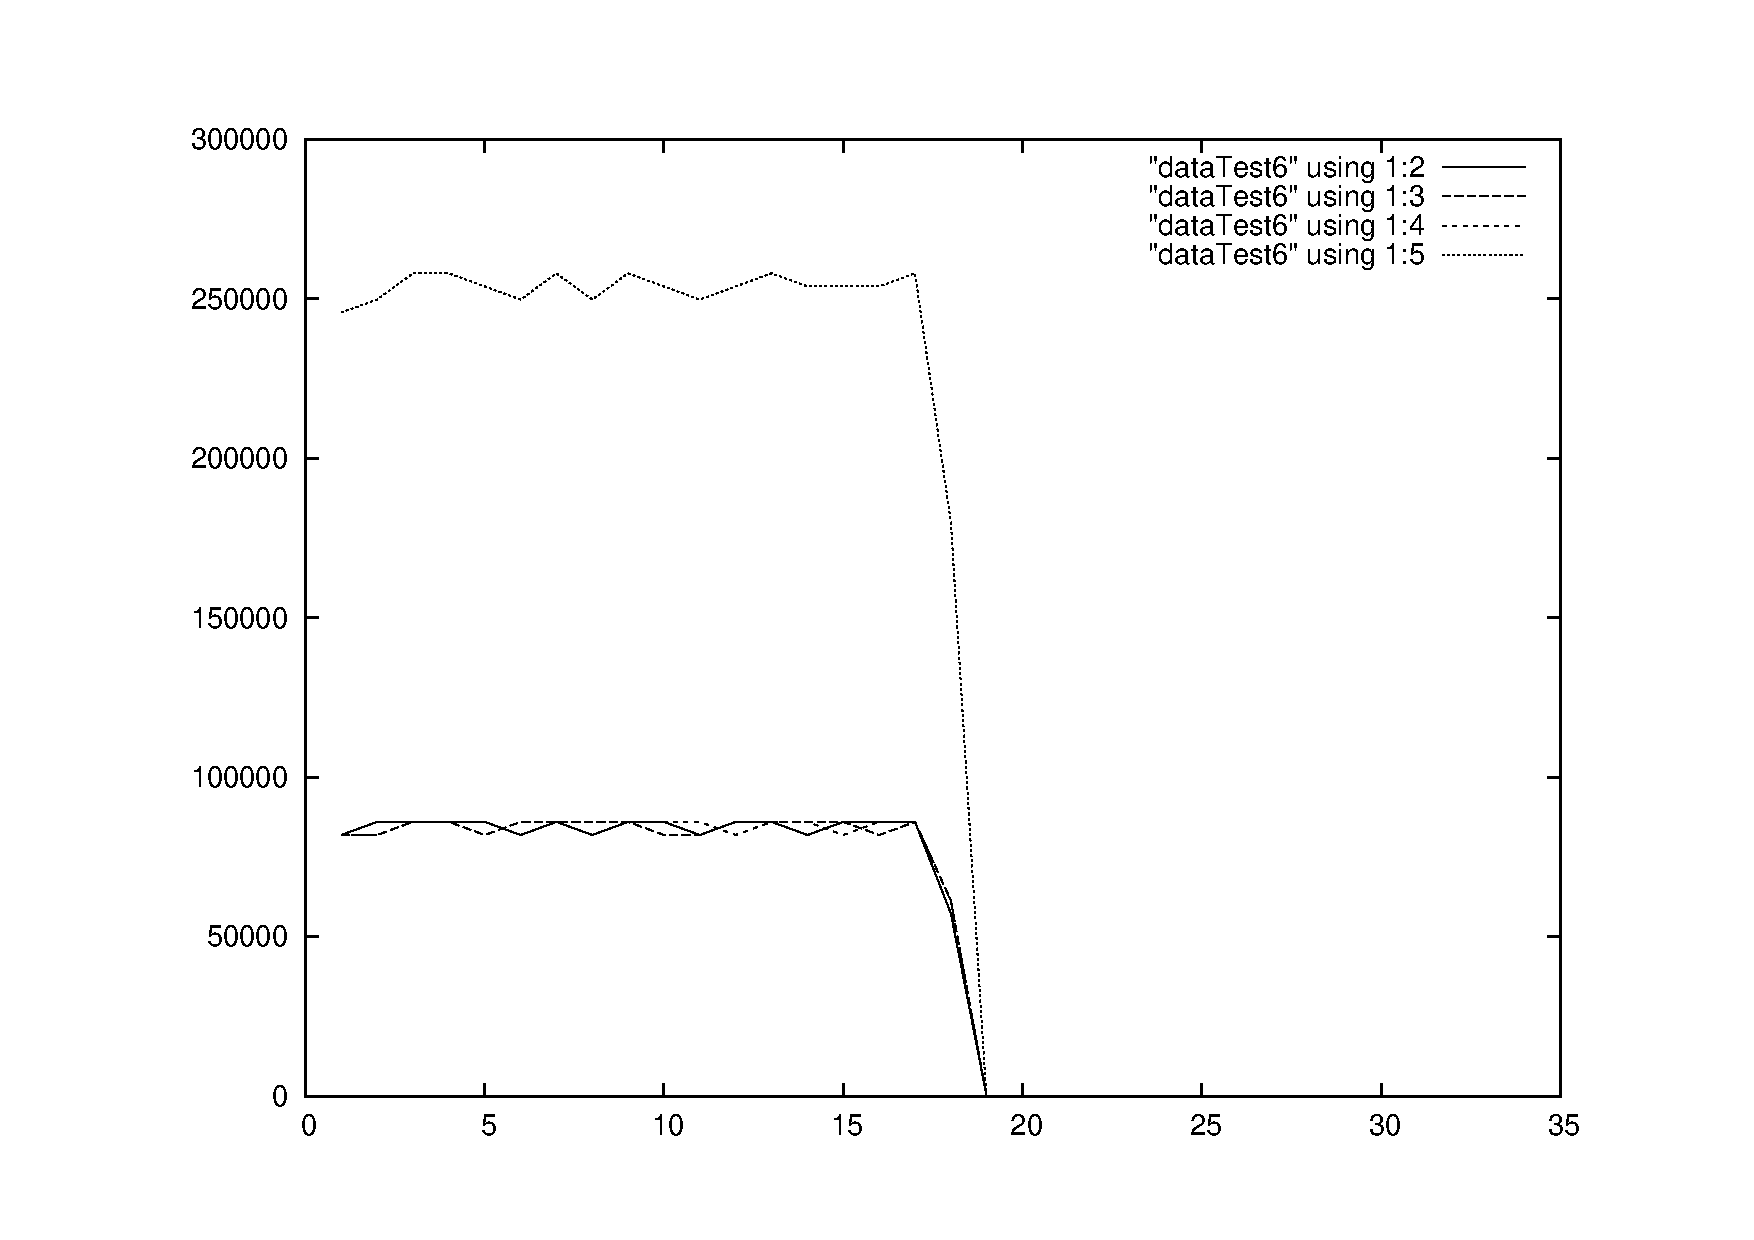
\includegraphics[width=3in]{plotTest6}}

{\centering PlotTest6.pdf\\}
{\centering The expected finish time is $1500000*3/250000 ~= 18 seconds$.
}



\section{Part 3: STFQNWScheduler}

{\em For part 3, we used one lock and one condition variable: okToSend, which signals 
that a buffer may quit waiting and proceed with its data send. As in part 2, we 
have maxRate and nextDeadline. 
However, in order to implement the STRQ algorithm, we added a few things. 
First off, we made a struct for buffers, that contains their startTag and finishTag. 
We also included a variable virtualTime, which keeps track of the scheduler's virtual 
time as described in the project description. We also keep track of the waitingBuffers, 
the maxFinishTag, and have an array to keep track of the previous finish tag per stream: 
prevFinishTag[$MAX\_FLOW\_ID + 1$]. To manage our buffers, we used a priority queue. To sort 
them by decreasing startTags, we overrode the $'<'$ operator.

Our implementation of waitMyTurn(...) followed the project specs very closely. We set the 
start and finish tags according to the formulas, set the maxFinishTag, and pushed the 
buffer onto our priority queue. We make the current buffer wait as long as the current 
time has not reached its prescribed deadline or the startTag of the current buffer does not 
match the startTag of the buffer on the top of the queue (which has the lowest startTag 
of all buffers on the queue). When the buffers is signalled from waiting, we set the new 
virtual time, nextDeadline, previous finish tag, and pop the buffer off of the queue. 

Our signalNextDeadline(...) function simply signals that it is ok for a buffer to send and 
returns nextDeadline.}

{\em For our testing strategy, we used a similar structure to that
of part 2. The primary difference is we changed
the number of threads to run, as well as the dieTime in util.cc. 
We also calculated predicted amount of seconds that each of the STFQ 
tests would last in terms of sending all of its bytes. 

Important: See the comments in the Makefile in the testPlot commands
(the comments show how many nflows will run as well at the maximum dieTime)}

{\em IMPORTANT: Our testing graphs included in this report were "made" with the specified 
nflows and dieTimes in the Makefile. If you wish to re-make the graphs, you must follow 
our directions in seeting nflows and dieTime in unit.cc. We have not included the command 
to make all of our graphs when you make report.pdf for this reason.}

\subsection{Evaluation}

\centerline{\includegraphics[width=3in]{plot3}}

{\em As we can see from the graph, there are 5 flows, each flow sending more bytes than the other. This is because a flow with a higher weight has the ability 
to send more bytes in accordance to the Start-Time Fair Queueing algorithm. In a similar sense to the MaxNWScheduler (plot2), because of the greatly large amount of 
bytes to send, it will take much longer than 30 seconds to see where in the graph the flows stop sending bytes.}

\centerline{\includegraphics[width=3in]{plot3b}}

{\em Now that we have a much lower amount of bytes to send, we can see what happens when the flows stop sending bytes. As you can see here, the flow with the highest weight (sending 300,000 bytes/second
will stop sending after ~16.66 seconds (5,000,000/300,000 = 16.6666). Once that flow stops sending, and amount of bytes sent of the other 4 flows increase. When the flow with highest flow at that time stops
sending, the 3 remaining streams will be able to send more bytes, and so on.}

\subsection{Our Test Result Graphs for STFQNWScheduler}

\centerline{\includegraphics[width=3in]{plotTest5}}

{\centering PlotTest5.pdf\\}
{\em The expected finish time is $600000*2/60000 ~= 20 seconds$.
}

\centerline{\includegraphics[width=3in]{plotTest7}}

{\centering PlotTest7.pdf\\}
{\em The expected finish time is $1500000*6/250000 ~= 36 seconds$.
}

\centerline{\includegraphics[width=3in]{plotTest8}}

{\centering PlotTest8.pdf\\}
{\em The expected finish time is $13500000*4/950000 ~= 56.8 seconds$.
}

\end{document}


